\documentclass[12pt]{article}

\usepackage{sbc-template}
\usepackage{graphicx,url}
\usepackage[brazil]{babel}
\usepackage[latin1]{inputenc}
\usepackage{lscape}
\usepackage{geometry}
\usepackage{float}
\usepackage{algorithm2e}
\usepackage{multicol}
\usepackage{amsmath}
\usepackage{amsfonts}
\usepackage{amssymb}
\usepackage{makeidx}
\usepackage{graphicx}
\usepackage{lmodern}
\usepackage{enumerate}
\usepackage{latexsym}
\usepackage{longtable}
\usepackage[all]{xy}
\usepackage{float}
\usepackage{lscape}
\usepackage{mathrsfs}
\usepackage{fancyhdr}
\usepackage{boxedminipage}
\usepackage{enumitem}


\sloppy

\title{Implementação do algoritmo k-NN}

\author{Marco Cezar Moreira de Mattos\inst{1}, Rômulo Manciola Meloca\inst{1}}

\address{DACOM -- Universidade Tecnológica Federal do Paraná (UTFPR)\\
  Caixa Postal 271 -- 87301-899 -- Campo Mourão -- PR -- Brazil
  \email{\{marco.cmm,rmeloca\}@gmail.com}
}

\begin{document}

	\maketitle

	\begin{resumo}
		Relata o procedimento tomado para implementar o algoritmo k-NN e os testes feitos com ele sobre um conjunto de dados.
	\end{resumo}

	\section{O algoritmo}\label{sec:algoritmo}
		
		O K-nearest neighbors (k-NN) é um algoritmo de classificação inteligente que avalia os k elementos mais similares ao elemento a que se deseja classificar e então rotula-o por meio de voto majoritário. É classificado como um algoritmo de aprendizagem supervisionada, de modo que exige um conjunto de treinamento já com as respostas de cada instância de treino.

		O k-NN pode calcular a proximidade de instâncias 

		\begin{algorithm}[H]
			\KwData{Conjunto de testes}
			\KwResult{Matriz de confusão}
			Insere a primeira instância na lista do caminho percorrido\;
			\While{Puzzle não está resolvido}{
				Obtém o última instância do caminho\;
				Obtém os possíveis movimentos da instância\;
				Calcula a heurística para cada possível movimento\;
				Escolhe a instância que possui melhor heurística\;
				Adiciona a instância ao caminho percorrido\;
			}
			\caption{Pseudo-código k-NN}
		\end{algorithm}

		Obviamente em um cenário real, ao ser empregado o algoritmo k-NN, 

	\section{Implementação}\label{sec:implementacao}


		meses do ano

		1200 instâncias para o conjunto de teste com 24 características
		teste controlado uma vez que possuem respostas

		3600 instâncias para o conjunto de treino com 24 características
		possui resposta uma vez que é um algoritmo supervisionado, isto é

		utilizou-se a distância euclidiana

		implementou-se em java.
		Diagrama de classes.

		\newgeometry{left=0cm,bottom=0cm,right=0cm,top=0cm}
		\begin{landscape}
		\centering
		\begin{figure}[p]
		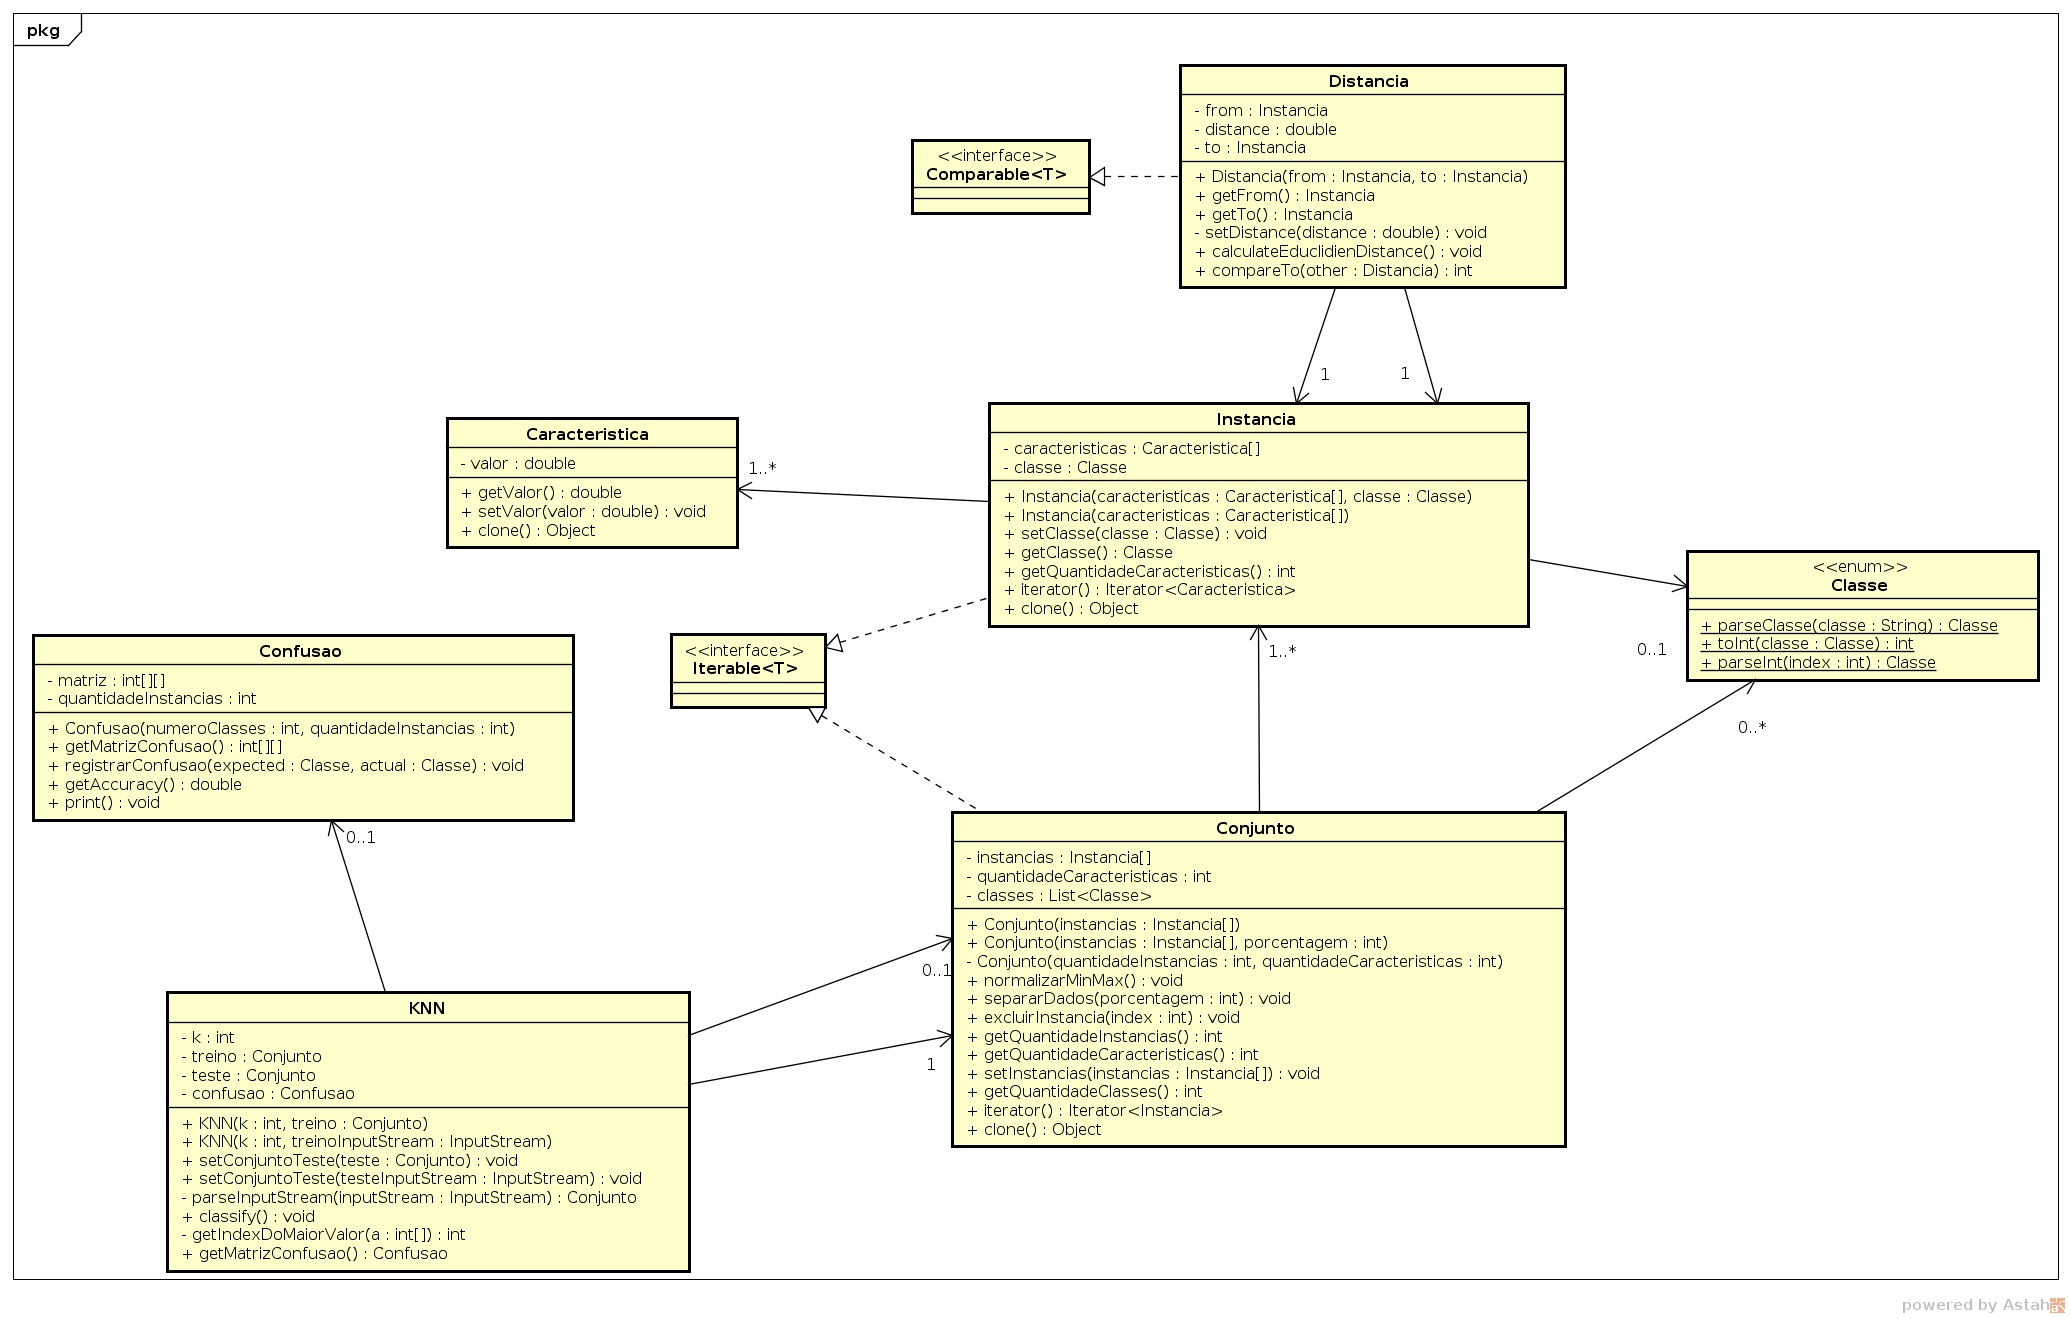
\includegraphics[width=1.4\textwidth]{classDiagram.png}
		\caption{Diagrama de Classes}
		\label{fig:classDiagram}
		\end{figure}
		\end{landscape}
		\restoregeometry

	\section{Teste}\label{sec:testes}

		\begin{itemize}
			\item Seu algoritmo deve avaliar o desempenho para diferentes valores de k;
			\item Gerar a matriz de confusão;
			\item Usar a distância Euclidiana, Manhattan ou outra;
			\item Normalizar os dados com Min-Max ou Z-score;
			\item Separar o conjunto de treinamento (aleatoriamente) em 25\%, 50\% e 100\% dos dados de treinamento. Avaliar qual o impacto de usar mais e menos instâncias no conjunto de treinamento.
		\end{itemize}


	\section{Considerações Finais}\label{sec:consideracoesFinais}

		

	\section{Referências}\label{sec:referencias}

		

\end{document}